The efficiency of the system is dependant on the torque through the gearbox as shown in Fig \ref{eff_results}.
This contradicts previous studies that suggested that cycloidal drives have a constant efficiency across the torque range.
There is also a much less pronounced relationship between the velocity and the cycloid efficiency that can be noted in the torque bands.
This result suggests that the cycloid efficiency behaves more like a planetary or harmonic drive gearbox in its efficiency profile.
A comparison of cycloid, harmonic, and planetary efficiency profiles can be seen in Fig \ref{eff_comp}.
The figure shows the efficiency for a harmonic drive CSF-45-50-2UH-LW \cite{harmonic_sheet} which has a comparable ratio and torque capability to the tested cycloid and weighs 5.1kg, and a representative planetary efficiency curve from the engineers at Maxon Motor.
If backlash is acceptable in a system, a cycloidal drive can provide similar or better efficiency profiles to a harmonic drive while providing a potential 2x increase in specific torque (Nm/kg).

\begin{figure}[t]
   \centering
   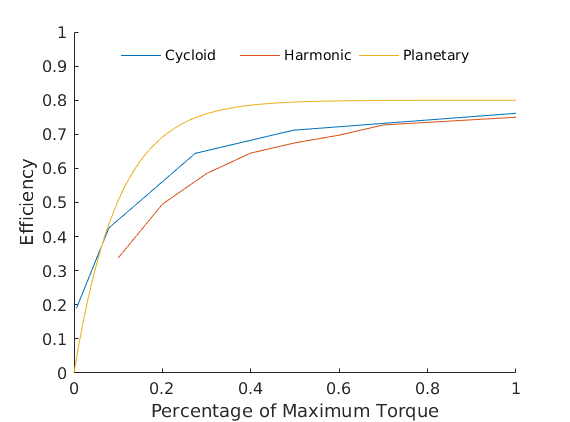
\includegraphics[width=\linewidth]{images/eff_comp_v3}
   \caption{Comparison of efficiency over maximum torque rating of the tested cycloid, a comparable harmonic drive, and a theoretical planetary gearset.
   The cycloid exhibits the same efficiency increase over torque range and has a comparable and slightly higher efficiency than the harmonic.}
   \label{eff_comp}
\end{figure}

There was a substantial break-in time for the actuator before steady state results were achieved (see Fig \ref{long_run}).
In the high torque case, specifically in the reverse direction, there was an approximately linear increase in efficiency over the course of the first seven hours of duty cycle testing.
This testing began after a minimum of five hours of run time spread out through many short sessions while getting the test system running.
The large increase in efficiency can be noted in the other lower torque profiles as well, starting well below their final steady state values.
The authors theorize that this is due to break-in of the manufactured parts required because of machining inaccuracies.
Due to the complex interaction required of the trochoidal motion profile, slight manufacturing deficiencies could cause build-ups of stress and loss in particular points on the drive.
It would make sense that these could manifest in one direction and not the other if a lobe was misshapen on the trailing edge in one direction, it would be the lead in the other, causing the additional loss.
Through the first hours of testing, these materials likely wore in to each other until the contact was smooth, resulting in the more readily achieved steady state efficiencies in subsequent hours of testing.

Additionally, there is a marked improvement over the first 30 minutes of runtime in the efficiency of the system.
This is likely due to the grease and heat in the system.
The gearbox is greased with Lucas Oil Red'N'Tacky which has a viscosity index of 86 min.
This was chosen because it is designed for high loads for extended periods of time in gear and sliding surface applications, as well as ease of use for Earth testing and verification.
Therefore, during the warm-up period as the actuator temperature increases, the viscosity decrease is likely enough to cause a notable increase in efficiency of the system.
The authors leave the study of a lower viscosity grease's effect on performance, as well as grease suitable for vacuum, for future work.

